\chapter{Revision Control}


\includegraphics[scale=0.20]{../images/owl-50267_1920.jpg}

\justify
The advantages of using a revision control\index{revision control} methodology in being able to
organize and store project artifacts in a way that multiple users or
teams can leverage. Websites, like github.com for example, are
fundamental to our workflow as they are a key piece of our software
delivery pipeline.

\justify
In addition to giving us a way to back up and store our work,
essentially for free, it facilitates a greater degree of collaboration.
There are other similar, (mostly) free services we can choose from
including Bit Bucket and Git Lab. For the purposes of this book we will
focus on the most well known of these, GitHub\index{GitHub}.

\section{github.com}

Simply put, github.com is a website that allows you to store the work
you are using git to manage. Git is the tool that allows for revision
control of your work. GitHub is a repository for storing that work,
creating teams to work on projects, tracking issues, release
snapshotting, and more.

\subsection{Enable Two-Factor Authentication}

\justify
One of the very first things you should do (after creating an account,
that is) is to configure two-factor authentication\footnote{\url{https://help.github.com/en/github/authenticating-to-github/securing-your-account-with-two-factor-authentication-2fa}}
(2FA) for your GitHub account.

single: two-factor authentication

\subsection{SSH Key Setup}

Take a few minutes to generate an SSH key\index{SSH keys} pair if you don't already have
one. We will be using it at various stages to log in to various sites
and hosts. The directions for generating an SSH keypair found on the
github.com website\footnote{\url{https://help.github.com/en/github/authenticating-to-github/generating-a-new-ssh-key-and-adding-it-to-the-ssh-agent}}
are perfect for this task.

\begin{mybox}{\thetcbcounter: SSH Key Generation}
ssh-keygen -t rsa -b 4096 -C "user@example.com"\\
Enter a file in which to save the key (/home/user/.ssh/id\_rsa): [Press enter]\\
Enter passphrase (empty for no passphrase): [Type a passphrase]\\
Enter same passphrase again: [Type passphrase again]
\end{mybox}

\justify
Now you can add your public key half to github.com\footnote{\url{https://help.github.com/en/github/authenticating-to-github/adding-a-new-ssh-key-to-your-github-account}}.

\subsubsection{GPG Key Setup}

\justify
Using a GPG key to sign your commits\footnote{\url{https://help.github.com/en/github/authenticating-to-github/generating-a-new-gpg-key}}
will help others verify that work you check in to revision control did
actually come from you. It's not strictly necessary but is considered
good practice. Some repositories require that you sign your pull
requests with your GPG key\index{GPG key}.

\justify
Take a few minutes to set up a GPG key and add it to your profile on
GitHub.

\begin{mybox}{\thetcbcounter: GPG Key Setup}
user@devsecops:\~\# gpg --default-new-key-algo rsa4096 --gen-key\\
public and secret key created and signed.\\
Note that this key cannot be used for encryption.  You may want to use
the command "--edit-key" to generate a subkey for this purpose.\\
pub   rsa4096 2020-05-12 [SC] [expires: 2022-05-12]\\
\hspace*{15mm}      848943CDCE488F138BF91079E81498874E59648D\\
uid\\
\hspace*{25mm}                     Kevin Flynn <user@example.com>\\

user@devsecops:\~\# gpg --list-secret-keys --keyid-format LONG |grep sec| cut -f2 -d'/'|cut -f1 -d' '\\
E81498874E59648D\\
user@devsecops:\~\# gpg --armor --export E81498874E59648D
\end{mybox}

Copy your GPG key, beginning with
-\/-\/-\/-\/-BEGIN PGP PUBLIC KEY BLOCK-\/-\/-\/-\/- and ending with
-\/-\/-\/-\/-END PGP PUBLIC KEY BLOCK-\/-\/-\/-\/-. Add the GPG key to
your GitHub account.

Next let's take a look at two of the key methods of interacting with
projects and other people on github.com.

\hypertarget{forking-and-cloning-repositories}{%
\subsubsection{Forking and Cloning
Repositories}\label{forking-and-cloning-repositories}}

When someone else has a project on github.com that you would like to
make changes to, you can make a "fork" of that project. Forking a
repository means you are making a copy of that repository to your
personal account on the GitHub web site.

single: Forking

Creating a "clone" of your fork to your local machine is done so that
you can make changes without altering the original project before
testing and reivew of the changes takes place.

single: Cloning

Adding a "remote" is a git convention to easily push changes from your
clone back to the original source repository.

\begin{description}
\item[digraph forking \{]
"Original Repository on github.com" {[}shape=rectangle{]}; "Your fork on
github.com" {[}shape=rectangle{]}; "Local Clone" {[}shape=rectangle{]};
"Original Repository on github.com" -\textgreater{} "Your fork on
github.com"{[}arrowhead=normal{]}; "Your fork on github.com"
-\textgreater{} "Local Clone"{[}arrowhead=normal{]}; "Local Clone"
-\textgreater{} "Original Repository on github.com"{[}arrowhead=normal
label="add remote called upstream"{]};
\end{description}

\}

This can be a tricky pattern to master, but it is fundamental if you
want to join the ranks of Open Source contributors and developers that
enjoy the full power of Git and GitHub.


\paragraph{Steps:}

\begin{itemize}

\item
  From the original project page on github.com, click the "fork" button.

  \begin{itemize}

  \item
    This creates a copy of the original repository on your personal
    GitHub page.
  \end{itemize}
\item
  Now from your page, make a clone of that fork from github.com to your
  machine.

  \begin{description}
  \item[- This will allow you to add, update and test code and
  documentation without]
  altering the original project.
  \end{description}
\item
  On your local machine, create a "remote" connection back to the
  original repo.
\end{itemize}

To create a "remote" called upstream from your clone to the original
repo, use this example command:

\begin{mybox}{\thetcbcounter: Create Upstream Remote}
git remote add upstream git@github.com:hotpeppersec/rapid\_secdev\_framework.git
\end{mybox}

After completing these steps you can easily submit pull requests (PRs)
back to the original project.

\hypertarget{keeping-a-clone-in-sync}{%
\subsubsection{Keeping a Clone in Sync}\label{keeping-a-clone-in-sync}}

The process of performing a pull request (PR) and merging changes is
covered fairly extensively on the Web. Let's take a quick look at how to
keep your local clone of a repository, as well as your clone on
github.com, up to date.

\hypertarget{steps-1}{%
\paragraph{Steps}\label{steps-1}}

These are the steps to take once your pull request is merged to the main
branch in the main project repository. From the command line on the
machine where your clone resides:

\begin{itemize}
\item
  git checkout master
\item
  git fetch upstream
\item
  git rebase upstream/master
\item
  git push origin master
\end{itemize}


\subsection{Creating Repositories}

\justify
If you are starting out on a new project, simply creating a repo is
probably enough. Often I will start a repository on my personal account
while I use the steps in this book to get the project of fthe ground.
Later I will move the repository into an organization where the
responsibility for ownership and administration can be shared with other
folks.

\justify
While the repository is owned by me, I use a much simpler process for
managing my code check-ins.

\hypertarget{steps-2}{%
\paragraph{Steps}\label{steps-2}}

\begin{itemize}

\item
  Create the repository on github.com from my personal account.
\item
  Make a clone of that new repository from github.com to my local host.
\item
  Do my pull requests and merges as desired.
\item
  Do a git pull to my master branch to keep my local clone up to date.
\end{itemize}


\subsection{Example Repository}

\justify
A GitHub Template Repository is available should you decide to follow
along with the code examples in this book. The next sets of steps are
predicated on having Docker installed and running as described in the
previous chapter.


\paragraph{Template Steps}

\begin{itemize}

\item
  Navigate to
  \url{https://github.com/hotpeppersec/rapid_secdev_framework}
\item
  Click the green button "Use this template"
\item
  Select a "Repository name", like "rapid\_secdev\_framework" for
  example.
\item
  Now click "Create repository from template"
\end{itemize}

\justify
Now you have a repository in your GitHub account that you can use for
testing and completing lab examples detailed in this book. For our first
exercise, let's try to make a clone of the repository we generated from
template.


\paragraph{Cloning Steps}

\begin{itemize}
\item
  Navigate to the main page for our new repository on github.com.
\item
  \begin{description}
  \item[Clone the repository to your local host by clicking on the green
  "Clone or download" button.]
  \begin{itemize}

  \item
    Be sure to clone with "SSH" and not "HTTPS".
  \end{itemize}
  \end{description}
\item
  Change to the clone directory with the "cd" command.
\end{itemize}

From the rapid\_secdev\_framework directory, execute the command
make docker to get to a command prompt within the container.

Consider the following example. Notice that the command prompt changes
to indicate that you have a BASH shell in the running container.

\begin{mybox}{\thetcbcounter: Output from make docker command}
user@devsecops:\~/rapid\_secdev\_framework\$ make docker\\
Building test env with docker-compose\\
docker-compose -f docker/docker-compose.yml build devsecops\\
Building devsecops\\
Step 1/3 : FROM python:3.9-buster\\
---> 4f7cd4269fa9\\
Step 2/3 : WORKDIR /home/secdevops\\
---> Using cache\\
---> 95dc84398bc2\\
Step 3/3 : RUN apt update; apt install -y apt-utils\\
---> Using cache\\
---> 83ea11278488\\
Successfully built 83ea11278488\\
Successfully tagged docker\_devsecops:latest\\
user@devsecops:/home/secdevops\#
\end{mybox}


\subsection{CODEOWNERS}

\justify
Creating a CODEOWNERS\index{CODEOWNERS} file\footnote{\url{https://help.github.com/en/github/creating-cloning-and-archiving-repositories/about-code-owners}}
is a good way to automatically tag folks in PRs to make them aware of
changes to certain files or folders in your projects.

\justify
In it's most basic form, the CODEOWNERS file in the .github directory
simply lists the file(s) and the owner(s) on a line together.

\justify
Consider this example where we add the @hotpeppersec to the CODEOWNERS
file.

\begin{mybox}{\thetcbcounter: Adding a user to CODEOWNERS file}
user@devsecops:/home/secdevops\# if [ ! -d ".github" ];then mkdir .github; fi\\
user@devsecops:/home/secdevops\# echo "* @githubusername">> .github/CODEOWNERS
\end{mybox}

In this example, the @githubusername user will be tagged as a reviewer
in all pull requests.


\subsection{The .gitignore file}
\justify
Use this file\index{.gitignore} to designate items that should be excluded from revision
control. This is useful for helping keep credentials and other secrets
out of the GitHub repository.

\justify
Consider the following example .gitignore file. This will prevent you
from checking in the .DS-Store that Macintosh creates in many folders.

\begin{mybox}{\thetcbcounter: Example .gitignore file}
root@cloudlab:\~/workspace/cloudlab\# echo ".DS\_Store" > .gitignore
\end{mybox}

\subsection{Working with Branches}

Naming your branches something useful is helpful (self documenting).

Let's look at how to create a branch

\hypertarget{steps-3}{%
\paragraph{Steps}\label{steps-3}}


\subsection{Pull Requests}

\justify
When you make changes on a local branch, say on your personal laptop,
you will eventually want those changes to flow back into the main
project. Opening a pull request\index{Pull Request} is a means of letting other people know
you've got a set of changes ready for review and potential
changes\footnote{\url{https://help.github.com/en/github/collaborating-with-issues-and-pull-requests/about-pull-requests}}.

\justify
Keeping pull requests smaller and more frequent makes it easier for your
peers to review your changes. It also means you will be less likely to
lose work.

\justify
Let's use our changes to the CODEOWNERS file to try making a change in
our clone of the repository in GitHub, then pushing that change up to
the repository.

\hypertarget{steps-4}{%
\paragraph{Steps}\label{steps-4}}

\begin{itemize}

\item
  Create a new branch, for example git checkout -b newbranch
\item
  Create the .github directory if it does not exist, then the CODEOWNERS
  file in that directory.
\item
  Use git to add the file to the commit: git add CODEOWNERS
\item
  Commit the file with git, git commit -S -m 'add CODEOWNERS file'
\item
  Push this commit to github.com, git push origin newbranch
\item
  Use the github.com website to open and merge the pull request.
\end{itemize}


\subsection{Repository Settings}

\justify
When setting up a new repository in my GitHub account, I always click
the Settings tab (with the little gear icon) and then choose the
"Branches" section. The Default branch gets set to "master". Clicking
the "Add Rule" button, entering "master" for the "Branch name pattern",
and then the green "Create" button sets up master as a protected branch.
Consider the following example {myFig2}.

\begin{figure}
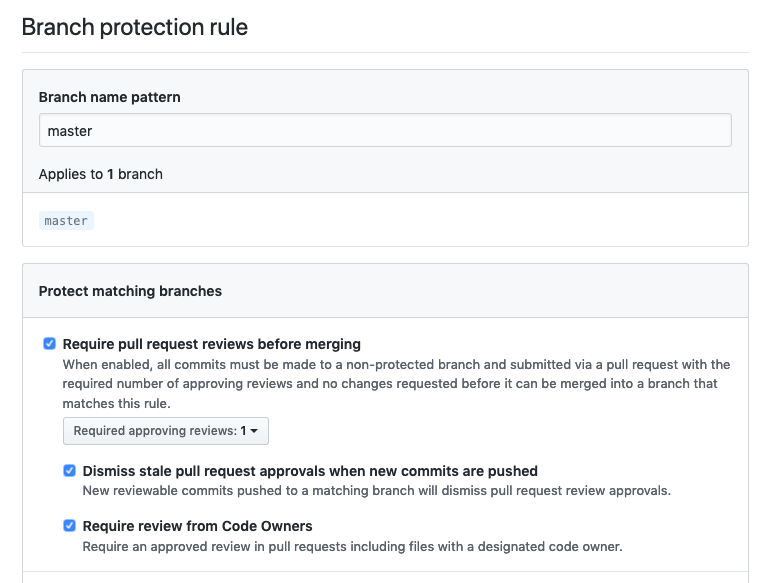
\includegraphics[scale=0.50]{../images/github-branch-protection.png}
\caption{Setting up branch protection.}
\end{figure}

\justify
After we start to work with CI/CD tools (status checks, like GitHub
Actions for example) new choices ({myFig3}) become available in this
part of your repository for managing those checks.

\begin{figure}
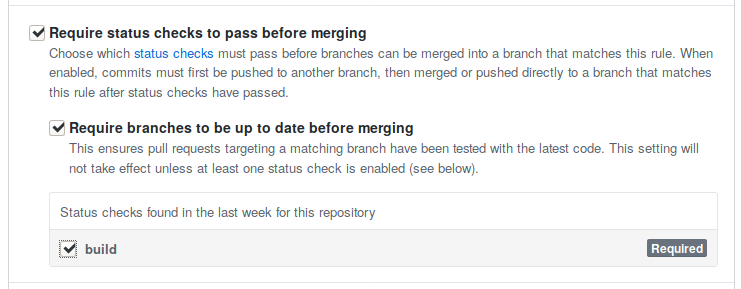
\includegraphics[scale=0.53]{../images/guthub-status-check.png}
\caption{Requiring status checks.}
\end{figure}

\subsection{Automated Repository Scanning}

\justify
There are many GitHub plugins that are free for
single-user/non-commercial scenarios. a cursory search of the web of the
GitHub Marketplace will turn up many of these. Let's leave some of the
tedious work to the bots so we can focus on our journey to the cloud!


\subsubsection{Renovate}

WhiteSource Renovate is what's known as a dependency scanner. It is free
for single user to add from the GitHub Marketplace\footnote{\url{https://github.com/marketplace/renovate}}
. It can tell you when you are using a version of a module or image that
is out of date. For example, if you have a Dockerfile that specifies
Python 3.8.1, Renovate will open a pull request on your repository to
update the version string in that Dockerfile to the most current version
available. You can also grant Renovate the permissions required to
simply merge the change with no human interaction. Renovate supports
JavaScript, Java, Ruby, PHP, Python, Go, Cargo, Elixir, Docker, and
more.

\justify
Once you've signed up and specified which repositories you want Renovate
to monitor, it opens a pull request to install a simple default
configuration file called renovate.json. Merge this initial pull request
and you're up and running!

\subsubsection{LGTM}

Semmle is a company that runs a code scanning service we can use to keep
an eye on our repositories for issues with syntax and dependencies. It
is tightly coupled with github.com and can be configured from lgtm.com
after logging in with your GitHub credentials.

\justify
As a fun aside, LGTM stands for "looks good to me", something developers
will add as review comments when their pull request is simple or matches
obvious expectations.

\clearpage


\section{Directory Structure}

Relevant files and folders mentioned in this chapter are organized as
seen below.

\begin{figure}
	\centering
	\digraph{githubdirectory}{
		size="8,4";
		node [fontname="Helvetica" fontsize=14 shape=box];
		edge [fontname="Symbol" fontsize=10];
		home [shape=folder fontname="Symbol" label="/home"]; 
		devsecops [shape=folder fontname="Symbol" label="/home/devsecops"];
		github [shape=folder fontname="Symbol" label=".github"];
		codeowners [fontname="Symbol" label="CODEOWNERS"];
		gitignore [fontname="Symbol" label=".gitignore"];
		home -> devsecops; 
		devsecops -> github;
		github -> codeowners;
		devsecops -> gitignore;
	}
	\caption{Project Directory and related files.}
\end{figure}
